Современный радиопередатчик состоит из следующих конструктивных частей (рисунок~\ref{fig:radiostruct})~\cite{wiki:radiotransmitter}:

\begin{itemize}
    \item задающий генератор частоты (фиксированной или перенастраиваемой) несущей волны;
    \item модулирующее устройство, изменяющее параметры излучаемой волны (амплитуду, частоту, фазу или несколько параметров одновременно) в соответствии с сигналом, который требуется передать (часто задающий генератор и модулятор выполняют в одном блоке — возбудитель);
    \item усилитель мощности, который увеличивает мощность сигнала возбудителя до требуемой за счёт внешнего источника энергии;
    \item устройство согласования, обеспечивающее максимально эффективную передачу мощности усилителя в антенну;
    \item антенна, обеспечивающая излучение сигнала.
\end{itemize}

\begin{figure}[ht]
    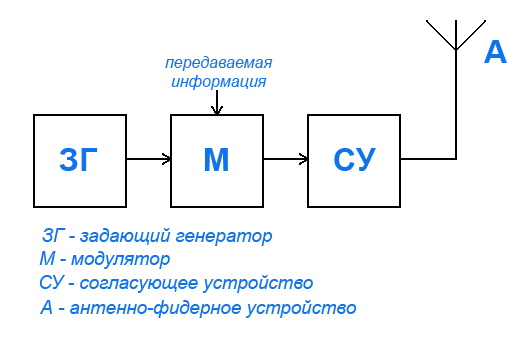
\includegraphics[width=.6\linewidth]{Figures/radiostruct.jpg}
    \caption{Структурная схема радиопередатчика}
    \label{fig:radiostruct}
\end{figure}

Принципиальная схема простейшего радиопередатчика представлена на рисунке~\ref{fig:rfcircuit}.

\begin{figure}[ht]
    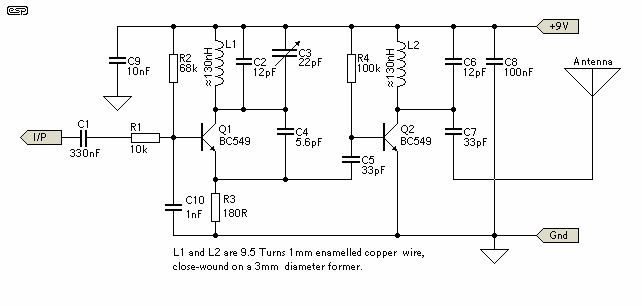
\includegraphics[width=1\linewidth]{Figures/rfcircuit.png}
    \caption{Простейшая принципиальная схема радиопередатчика}
    \label{fig:rfcircuit}
\end{figure}
